
\documentclass[
  english,        % define the document language (english, german)
  font=times,     % define main text font (helvet, times, palatino, libertine)
  onecolumn,      % use onecolumn or twocolumn layout
]{tumarticle}


% load additional packages
\usepackage{lipsum}
\usepackage{csquotes}
\usepackage[style=numeric-comp,sorting=none]{biblatex}
\usepackage{graphicx}
\usepackage{amsmath}
\usepackage{subcaption}

\addbibresource{resources/literature.bib}


% article metadata
\title{Time stepping review of open-source solvers}
\subtitle{Guided research}

\author[email=marc.amoros@tum.de]{Marc Amorós}

\date{
    \small
    \textbf{Supervisor:} Prof. Dr. Hans-Joachim Bungartz \\
    \textbf{Advisor:} M.Sc. Benjamin Rodenberg \\
}

\begin{document}

\maketitle

\begin{abstract}
    The accurate numerical simulation of physical phenomena is crucial in various scientific and engineering disciplines, and open-source solvers offer flexibility and accessibility to research and practitioners. A vital aspect of these solvers is the order of the time stepping scheme employed to evolve the solution over time, as it significantly affects the error of the obtained solutions. This work investigates and verifies the order of different time stepping methods implemented on various solvers. We focused on higher-order methods, which give better accuracy and help reduce the computational costs of obtaining a precise enough solution. To inspect the order of fluid-structure interaction (FSI) simulations using preCICE, we chose OpenFOAM and CalculiX as the studied solvers, which are compatible with this coupling library. 

    We observed a higher-order convergence when using second-order methods in single-solver simulations on both solvers and confirmed the correct convergence of first-order methods on FSI simulations. Moreover, we tested higher-order time stepping schemes on FSI simulations, which gave sub-linear error convergence. We followed by ruling out possible causes of this poor convergence and proposing possible solutions, making this work valuable for future projects aiming to obtain accurate FSI simulations in the preCICE environment.
\end{abstract}

\section{Introduction}
In scientific and engineering simulations, the precise numerical representation of physical phenomena is crucial for advancing knowledge and solving practical challenges. Open-source solvers have emerged as indispensable tools, offering flexibility and accessibility to researchers and practitioners alike. These solvers offer different time stepping schemes, and selecting one to evolve the solution over time is a decision that profoundly influences the error of the obtained solutions. This project investigates and verifies various time stepping methods implemented on different open-solvers, focusing on higher-order schemes.
    
Higher-order methods not only promise enhanced accuracy but also hold the potential to mitigate computational costs, which is crucial for obtaining precise solutions within reasonable time frames. Our study analyses if these claims hold for two specific open-source solvers and presents scenarios where higher-order convergence can be achievable. 

One can differentiate between single or multi-physics simulations. The first group target a specific domain, such as fluid dynamics, structural mechanics, heat transfer, or electromagnetics. The solvers of said simulations focus on solving equations specific to their respective domains and are often tailored to efficiently handle the complexities of that particular physics. On the other hand, multi-physics solvers integrate multiple physical domains into a single simulation framework. 

We selected OpenFOAM \cite{weller1998tensorial} and CalculiX \cite{calculix-web} as our fluid mechanics and structural solvers, respectively, given that they are widely used in industry and research, renowned for their reliability and good documentation. Moreover, both are compatible with the multi-physics coupling library preCICE \cite{preCICEv2}, which allowed us to compute fluid-structure interaction (FSI) simulations using both solvers as black boxes. This way, we could combine fluid dynamics and structural mechanics solvers to predict the dynamic behavior of structures immersed in fluid flows.

In the subsequent sections, we show how higher-order convergence is achievable in single-solver simulations using second-order methods. Furthermore, we couple the two single-physics solvers in an FSI simulation and observe how a linear convergence can be achieved with first-order time stepping methods. Contrarily, we display how using a second-order method does not improve but worsens the error convergence.

For transparency and reproducibility, all code utilized in this project is accessible via our repository at: \url{https://github.com/atmarc/guided_research}. 

\section{OpenFOAM}
OpenFOAM is an open-source computational fluid dynamics (CFD) software package widely used for simulating and analyzing complex fluid flow problems. Its solver modules employ finite volume methods to numerically solve the Navier-Stokes equations, making it a versatile tool for simulating fluid dynamics in various engineering and scientific applications. In this section, we will explain the convergence analysis performed to verify that it has a higher-order convergence in time.   

\subsection{Time stepping schemes}\label{sec:euler}
This solver offers various time stepping schemes, and we focused on two for our analysis. The first one is the Euler implicit scheme. Given the following partial differential equation:

\begin{equation}
    \frac{\partial u}{\partial t} = F(u, t)
\end{equation}
the Euler implicit scheme would discretize it as follows:

\begin{equation}
    \frac{u^{n+1} - u^n}{\Delta t} = {F}(u^{n+1}, t^{n+1})
\end{equation}
it is a first-order method that is relatively stable, which is why it is usually the default choice. For the purpose of this study, we also chose a second-order scheme, this being the Crank-Nicolson method \cite{crank1947practical}. This scheme combines an explicit and an implicit Euler step, leading to a second-order convergence in time. This method would discretize the previous PDE as: 

\begin{equation}
    \frac{u^{n+1} - u^n}{\Delta t} = \frac{1}{2} \left[F(u^n, t^n) +  F(u^{n+1}, t^{n+1}) \right]
\end{equation}
OpenFOAM uses a slightly different version of this method by introducing a blending coefficient $\theta$ between the Euler implicit and Crank-Nicolson methods. If $\theta = 0$, then we obtain the implicit Euler method, and if $\theta = 1$, then it's Crank-Nicolson. For stability, the value $\theta = 0.9$ is recommended in their documentation.

\begin{equation}
    \frac{u^{n+1} - u^n}{\Delta t} = \frac{\theta}{2} F(u^{n}, t^{n}) + \left( 1 - \frac{\theta}{2} \right) F(u^{n+1}, t^{n+1})
\end{equation}


\subsection{Convergence study}

To study the convergence behaviour of OpenFOAM, we focused on the Taylor-Green vortex \cite{taylor1937mechanism, chorin1968numerical}, a standard setup in CFD to validate fluid flow solvers, given that an analytical solution of the case is known. In a 2D, this solution can be obtained by the formulas:
\begin{align}
    &u(x, y, t) = -\cos(x) \sin(y) e^{-2\nu t} \\
    &v(x, y, t) = \sin(x) \cos(y) e^{-2\nu t} \\
    &p(x, y, t) = -\frac{1}{4}\left[\cos(2x) + \sin(2y)\right]e^{-2\nu t}
\end{align}
where $u$ and $v$ are the horizontal and vertical velocities respectively, $p$ is the pressure and $\nu$ is the viscosity of the fluid. This solution holds for a square domain of size $2\pi$. In Figure \ref{fig:taylor-green} we can see an example of the computed initial velocities. 

\begin{figure}[!ht]
    \centering
    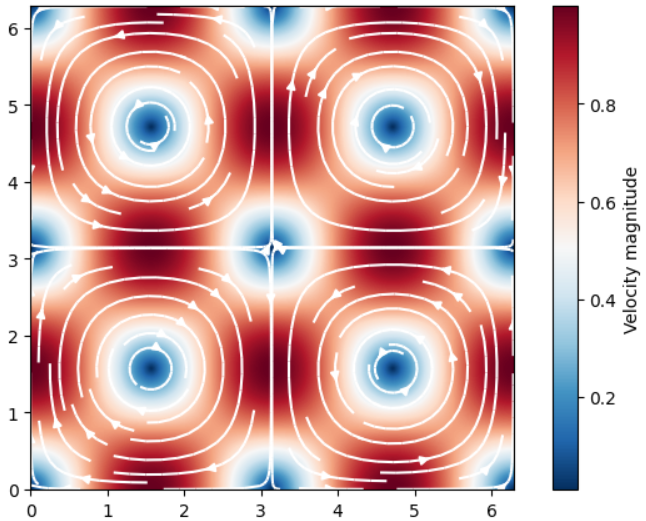
\includegraphics[width=0.5\textwidth]{resources/taylor-green-vortex.png}
    \caption{TODO}
    \label{fig:taylor-green}
\end{figure}

We implemented a program that computes the initial velocity for this setup, and writes it into the OpenFOAM configuration. We also wrote a script to automatize the configuration and execution of different setups with varying parameters, so we can perform several experiments automatically.
To observe the behaviour of the error, we did several executions of our setup case, fixing all the parameters (grid size, initial velocity, solver tolerances etc.) and changing the time step size. On our analysis, we mainly focused on the velocity profile.

In a simulation, there are several elements that contribute to the error $\varepsilon_{u}$. In this study, we were only interested in the error contribution of the time discretization scheme $\varepsilon_{\Delta t}$ to verify the order of the scheme. We assume that the error is formed by $\varepsilon_u = \varepsilon_{\Delta t} + \varepsilon_{\Delta x} + \varepsilon_\text{num}$, where $\varepsilon_{\Delta x}$ is the spatial discretization error, and $\varepsilon_\text{num}$ is the error introduced by numerical errors, and other factors. We know that $\varepsilon_{\Delta x}$ is related to the grid size, so we can assume that is constant among the experiments with the same grid size.

\begin{figure}[!htbp]
    \centering
    \begin{subfigure}[b]{0.49\textwidth}
      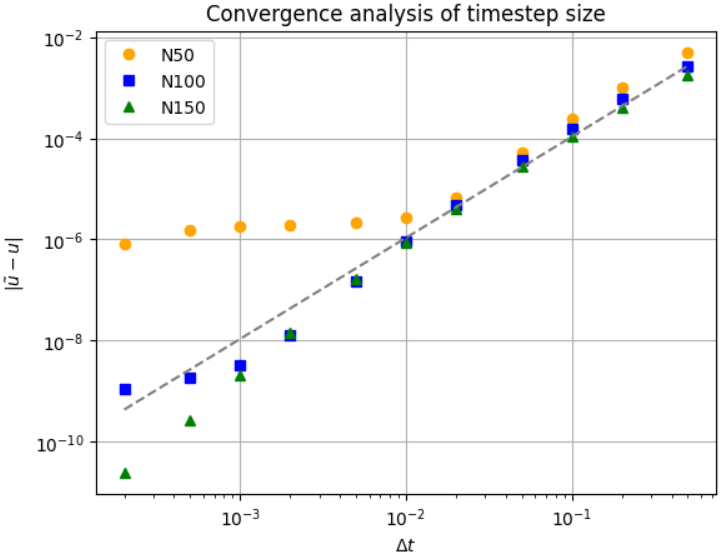
\includegraphics[width=\textwidth]{resources/convergence_study_openfoam.png}
      \caption{}
      \label{fig:convergence_openfoam}
    \end{subfigure}
    \hspace{1pt}
    \begin{subfigure}[b]{0.49\textwidth}
        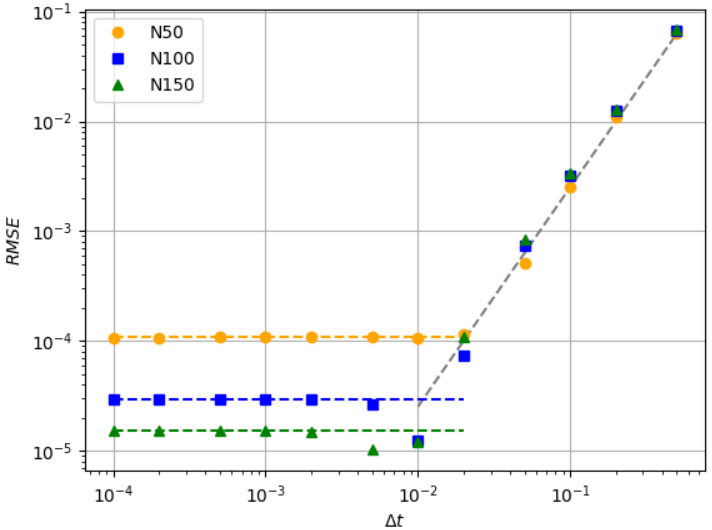
\includegraphics[width=\textwidth]{resources/RMSE_study.png}
      \caption{}
      \label{fig:RMSE_openfoam}
    \end{subfigure}
    \caption{TODO: Caption for both figures}
    \label{fig:figures}
  \end{figure}
  


There are several possible approaches to study the error. Our strategy was to choose a position cell $(i,j)$ and compare the values of the cell in this position for the different samples. We define as the reference sample $\tilde{u}$, obtained by running the simulation with a $\Delta t = 10^{-5}$. 
We computed the absolute difference between every sample and the chosen reference solution $|u - \tilde{u}|$ and we plotted them in Figure \ref{fig:convergence_openfoam}, for three different grid sizes. As we assumed that $\varepsilon_{\Delta x}$ is constant among the samples with the same grid size, in this plot we obtain $\varepsilon_{\Delta t} + \varepsilon_\text{num}$, allowing us to extract conclusions form the convergence behaviour of $\varepsilon_{\Delta t}$. We can observe how the error decreases when the timestep gets smaller, proportionally to $\mathcal{O}(\Delta t^2)$, until a point where the error flattens. Our assumption is that this happens when $\varepsilon_{\Delta t} < \varepsilon_\text{num}$, and after a certain point this $\varepsilon_\text{num}$ dominates the entire error. It is also remarkable to see how this point of flattening happens on smaller timesteps for increasing resolutions of the domain.

As me mentioned before, the Taylor–Green vortex scenario has an analytical solution $u^*$, what allows us to obtain the exact error $\varepsilon_{u}$ of the solutions we obtained, as those are going to be of the form $u = u^* + \varepsilon_{u}$. To compute this error $\varepsilon_{u}$, we compute the root-mean-square error (RMSE) of the the velocity flow field, compared to the analytical solution as follows:  

\begin{equation}
    \text{RMSE} = \sqrt{\sum_{(i,j)} (u^*_{ij} - u_{ij})^2 }
\end{equation}

This is being plotted in Figure \ref{fig:RMSE_openfoam}, where once again we can observe the error decreasing proportionally to $\mathcal{O}(\Delta t^2)$, showing once again a second order convergence in time. In this Figure is very visible the flattening of the error, and how it happens in different points for different resolutions of the domain. This is given that, in this case, the flattening occurs when $\varepsilon_{\Delta t} < \varepsilon_{\Delta x}$, as this time the spatial error is included. This plot also clearly shows how this spatial error decreases for higher domain resolutions, and gives a clear idea of the magnitude of this $\varepsilon_{\Delta x}$ in these scenarios. 


\section{CalculiX}\label{sec:calculix}
CalculiX is an open-source finite element software suite primarily used for solving structural analysis problems. It is designed to simulate the behavior of mechanical and structural systems subjected to various loading conditions. CalculiX provides capabilities for linear and nonlinear static, dynamic, and thermal analyses. It supports a variety of element types, boundary conditions, and material models, making it suitable for a wide range of engineering simulations. In this section, we will overview the timestepping scheme implemented in the solver, and present the convergence study we performed, that displays a higher order convergence. 

\subsection{Time stepping scheme}\label{sec:alpha}
The only time stepping scheme implemented in CalculiX is the $\alpha$-method \cite{dhondt2017calculix}. The solver allows the user to select between an implicit or an explicit version of it, and allows to control the $\alpha$ parameter. Moreover, one can define a fixed timestep size, using the DIRECT clause. To get an idea of how this method works, we can start with a given material point with displacement $\boldsymbol{u}$, velocity $\boldsymbol{v}$ and acceleration $\boldsymbol{a}$. We know that the acceleration and velocity are related as such $\boldsymbol{a} = \dot{\boldsymbol{v}}$, and this yields to the following formula to obtain the next timestep values:
\begin{equation}
    \boldsymbol{v}^{n+1} = \boldsymbol{v}^n + \int_{t^n}^{t^{n+1}} \boldsymbol{a(\xi)} \text{d}\xi
\end{equation}
The integral on the right-hand side can be aproximated by a linear combination of $ \boldsymbol{a}^n$ and $\boldsymbol{a}^{n+1}$:
\begin{gather}
    \boldsymbol{a}(\xi) \approx  (1 - \gamma) \boldsymbol{a}^n + \gamma \boldsymbol{a}^{n+1}\\
    \boldsymbol{v}^{n+1} = \boldsymbol{v}^n + \Delta t \left[ (1 - \gamma) \boldsymbol{a}^n + \gamma \boldsymbol{a}^{n+1} \right]
\end{gather} 
A similar reasoning can be applied to $\boldsymbol{u}$, as $\boldsymbol{\dot{u}} = \boldsymbol{v}$, hence:
\begin{equation}
    \boldsymbol{u}^{n+1} 
    = \boldsymbol{u}^n + \int_{t^n}^{t^{n+1}} \boldsymbol{v(\eta)}  \text{d}\eta 
    = \boldsymbol{u}^n + \Delta t \boldsymbol{v}^n + \int_{t^n}^{t^{n+1}} \int_{t^n}^{\eta} \boldsymbol{a(\xi)} \text{d}\xi \text{d}\eta 
\end{equation}
Assuming again that we can approximate $\boldsymbol{a}$ by a linear convination of $ \boldsymbol{a}^n$ and $\boldsymbol{a}^{n+1}$ in the interval $\left[ t^n, t^{n+1} \right]$, we can compute the new displacement $\boldsymbol{u}^{n+1}$ as:
\begin{gather}
    \boldsymbol{a}(\xi) \approx  (1 - 2\beta) \boldsymbol{a}^n + 2\beta \boldsymbol{a}^{n+1}\\
    \boldsymbol{u}^{n+1} = \boldsymbol{u}^n + \Delta t \boldsymbol{v}^n
    + \frac{1}{2} (\Delta t)^2 \left[ (1 - 2\beta) \boldsymbol{a}^n + 2\beta \boldsymbol{a}^{n+1} \right]
\end{gather} 
Notice how the linear combinations can be different, so $2\beta \neq \gamma$. This is the basic setup of the $\alpha$-method, which is proven to be second-order accurate and unconditionally stable for $\alpha \in [-1/3, 0]$, if $\gamma$ and $\beta$ satisy that \cite{dhondt2004finite}:

\begin{align}
    \beta &= \frac{1}{4}(1 - \alpha)^2 \\
    \gamma &= \frac{1}{2} - \alpha
\end{align}
This $\alpha$ parameter controls the high frequency dissipation, and in CalculiX the value set by default is $\alpha=-0.05$.

\subsection{Convergence study} \label{sec:convstudycalc}
In this case, we simulated a solid elastic flap fixed to the floor. A constant force is applied perpendicular to the flap, which is initially resting, which makes it oscillate due to its elasticity. This scenario can be seen in further detail in the solid part of the preCICE perpendicular-flap tutorial \cite{perpendicularFlap} or in the code repository of this project.

\begin{figure}[!ht]
    \centering
    \begin{subfigure}[b]{0.5\textwidth}
        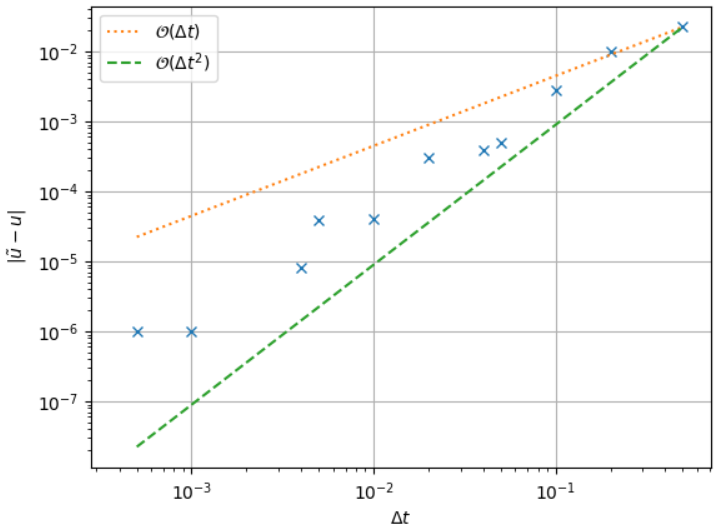
\includegraphics[width=\textwidth]{resources/calculix_convergence_study.png}
        \caption{TODO: .}
    \end{subfigure}
    \hspace{0.8cm}
    \begin{subfigure}[b]{0.35\textwidth}
        \raisebox{0.11\height}{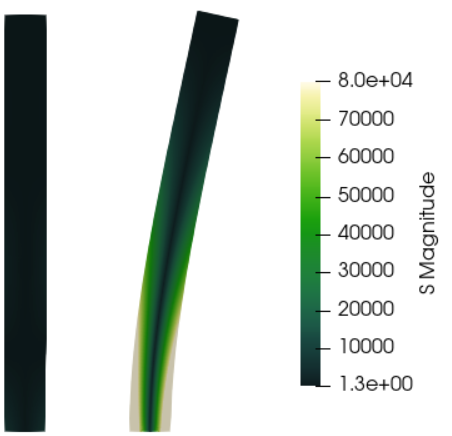
\includegraphics[width=\textwidth]{resources/elastic-flap.png}}
        \caption{}
    \end{subfigure}
    \caption{On figure b) we have an example simulation of the elastic flap, showcasing it's elasticity and the displacement of the tip. The colorscale represents the stress of the material.}
    \label{fig:calculix_convergence}
\end{figure}

Given the oscillatory behaviour of the flap, we measured the displacement of the flap's tip over time and used this value for the convergence study. As before, we implemented a script to automatize the execution of the simulations and the post-processing of the output data. We defined a reference solution $\tilde{u}$ as with the OpenFOAM study, which is the one obtained with a $\Delta t = 5\times 10^{-4}$. The output data format of CalculiX only has 6 significant digits, even though the solver works with double precision values. This means that we could obtain an output with better precision by modifying the solver's routines to export the data, but that rests out of the scope of this work. To circumvent this issue, we defined the simulation parameters so the error was significant enough to be visible in this precision range. This translates to a constant 10N force is applied in the X axis direction, and we take the measurements at $t=2s$. Then, we plotted the absolute difference to the reference solution $|u - \tilde{u}|$ to observe how the error behaves relative to this solution. One can see in Figure \ref{fig:calculix_convergence} how the error decreases faster than $\mathcal{O}(\Delta t)$. With the obtained results, one can definetly argue that the error follows a higher-order convergence, which in certain regions closely follows a second-order convergence. It is also noticeable how for smaller timesteps, the error gets more oscilatory, something that can happen due to the accumulation of other sources of error over time. 


\section{Coupling the two solvers} \label{sec:FSI}
% \begin{itemize}
%     \item Supported time stepping schemes, difference between v2 and v3 (window-size).
%     \item Talk about the parameters of the two solvers (mainly the same as the previous simulations, except change of openFOAM solver). 
%     \item Mention the possible preCICE parameters (coupling scheme?, ...).
% \end{itemize} 

We have observed on the previous sections how a higher order convergence is achievable with the OpenFOAM and CalculiX solvers. In this section, we will test them in a coupled simulation making use of the preCICE coupling library. To do so, we make use of the perpendicular flap setup that can be found on the example tutorials of the library \cite{perpendicularFlap}. It consists of two components, a two-dimensional fluid flowing through a channel, and a solid, elastic flap fixed to the floor of this channel. The fluid and solid parts of the simulation are computed by OpenFOAM and CalculiX respectively, comunicating between them with the help of preCICE. An example of this setup can be seen in Figure \ref{fig:FSI}.

\begin{figure}[!ht]
    \centering
    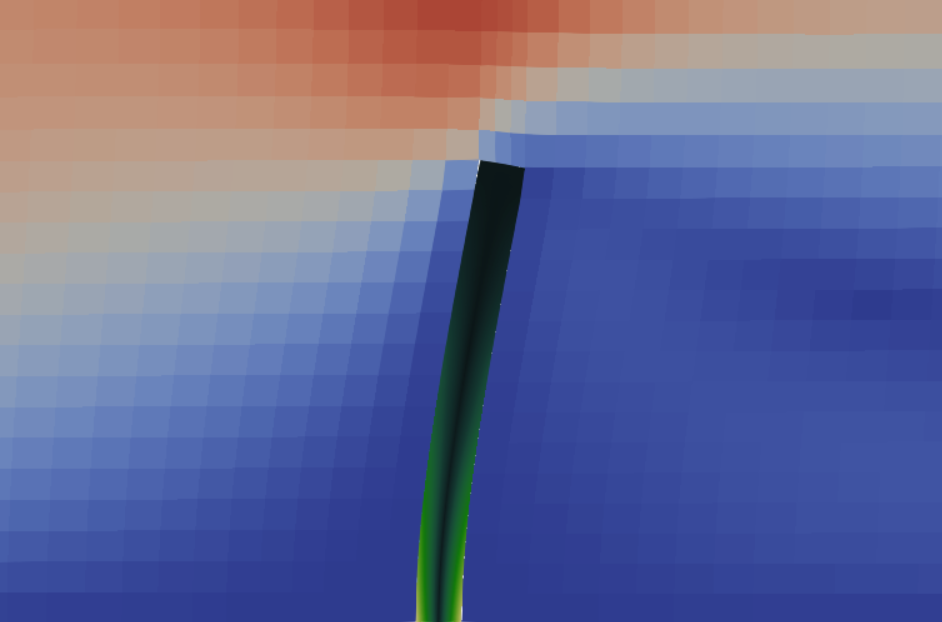
\includegraphics[width=0.45\textwidth]{resources/FSI_small.png}
    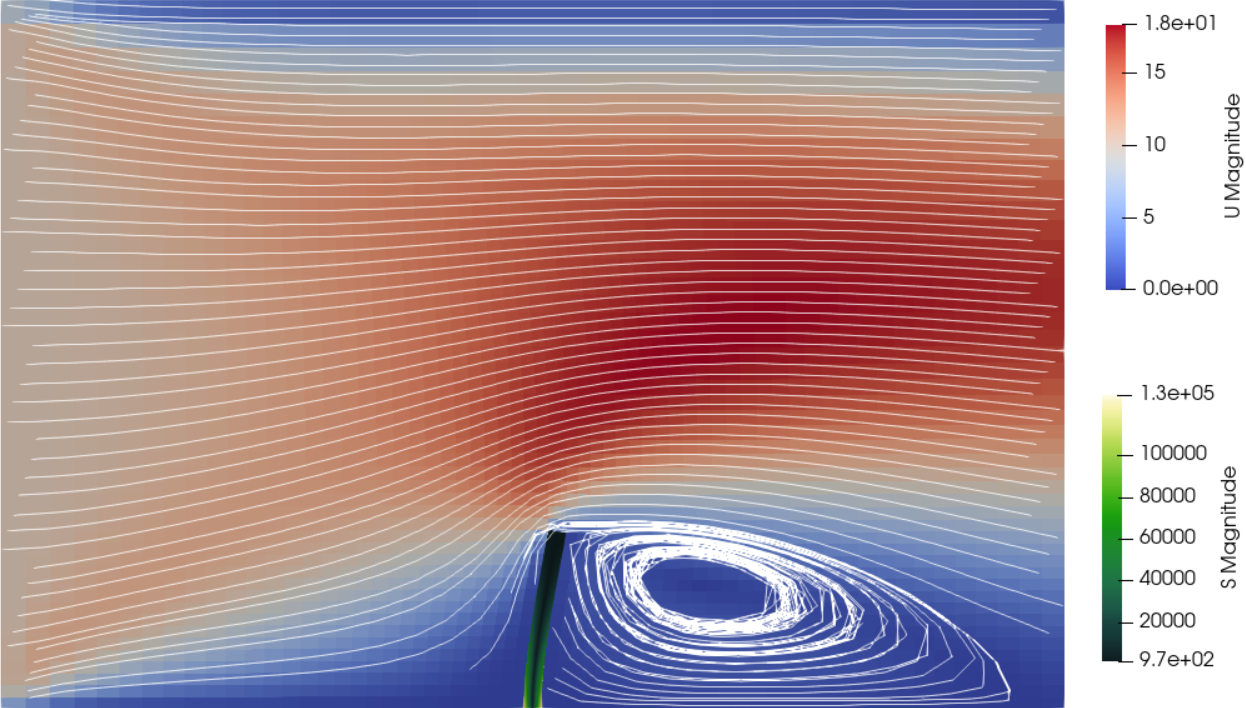
\includegraphics[width=0.53\textwidth]{resources/FSI_big.png}
    \caption{Example solution of the FSI simulation. The left image shows the zoomed in flap, where the stress of the material can be seen in a green scale. On the right image, we observe the whole domain, where we see the magnitude of the velocity field.}
    \label{fig:FSI}
\end{figure}

The flap oscillates due to the fluid pressure building up on its surface during a limited period, given by its initial resting position. The oscillations dampen until the entire system reaches a steady state. We will quantify the error of the simulation by measuring the displacement of the tip of the flap at time $t=1s$, which is still in oscilatory behaviour. We wrote specific scripts once again to automatize this task, utilizing similar solver parameters than in the previous sections. 

We ran multiple simulations setting the same timestep size on both solvers, and on the preCICE configuration. We also used both the Euler and Crank-Nicolson schemes, introduced in section \ref{sec:euler} for the fluid solver, to observe the difference on their error convergence. Moreover, we ran tests with the stable version 2 and the newest version 3 of preCICE, to observe if the update of the library affected the overall error. 
\begin{figure}[!ht]
    \centering
    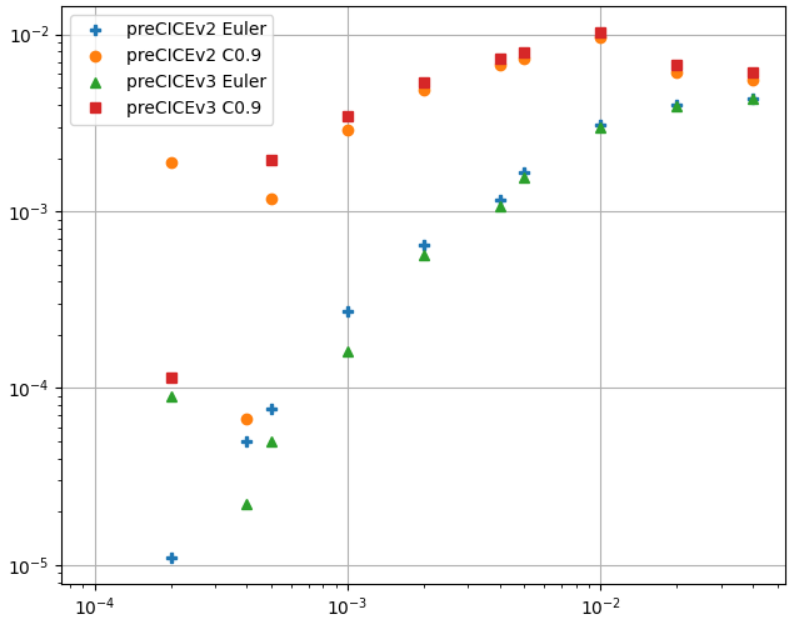
\includegraphics[width=0.5\textwidth]{resources/coupled_v2_v3_results.png}
    \caption{TODO: add title and maybe convergence lines}
    \label{fig:coupled_v2_v3}
\end{figure}
In Figure \ref{fig:coupled_v2_v3} we can observe the results of this experiments. One can observe how using the Euler method, we can achieve a first order convergence of the error. On the other side, we see how the Crank-Nicolson method performs poorly in this scenario, giving a worse convergence than the first-order method. It is relevant to mention how the different versions of the code seem to give different results, even though it does not affect the convergence behaviour.  

The reasons for the poor convergence of the second-order method can be various. preCICE is a complex environment with many moving many pieces. Each solver has its own adapter, that enables it to be a participant in a partitioned multi-physics simulation. This translates in many possible sources of error. In the next sections we rule out possible sources of error, and propose possible elements that could cause it. 


\section{Possible sources of error}
This section aims to identify and address the potential sources of error we encountered while coupling OpenFOAM and CalculiX using the preCICE library. On section \ref{sec:FSI} we observed that using a second-order time stepping method on the fluid solver, gave worse error convergence than using a first-order scheme, despite that both single solver analysis showed higher-order convergences. There are many possible sources of error in this case, starting by the preCICE components. To make sure that the component to blame is not the solid participant, we will test its correct behaviour while coupled to a dummy implementation of the fluid participant. Moreover, we will also test the fluid participant in section \ref{sec:fluid-part}.
% TODO: finish this text


\subsection{Verification of CalculiX adapter}
To interact with a participant solver, preCICE makes use of an adapter, which is an interface between the solver and the preCICE library. To verify the correct behaviour of one of this adapters, one can use a dummy implementation of another participant that only returns some preset magnitudes, and couple both using preCICE.

To test the correct behaviour of the CalculiX adapter \cite{yau2016conjugate}, we implemented a fake fluid script that could be coupled with CalculiX using preCICE. This fake fluid \cite{pullrequestfake-fluid} participant applied a force on the flap with the direction of the positive x axis, substituting what the OpenFOAM solver would produce on the FSI interaction. In this scenario, the returned force by the fake fluid was not constant but varying over time, following $f^n = f_{max} \sin(t^n + \phi)$ on the tip, and decreasing linearly over the height of the flap until reaching a 0 magnitude in the bottom. Our aim was to approximate the forces applied by the fluid on the flap, while making them time dependent to observe a pronounced decrease of the error with a higher-order time stepping scheme.

\begin{figure}[!ht]
    \centering
    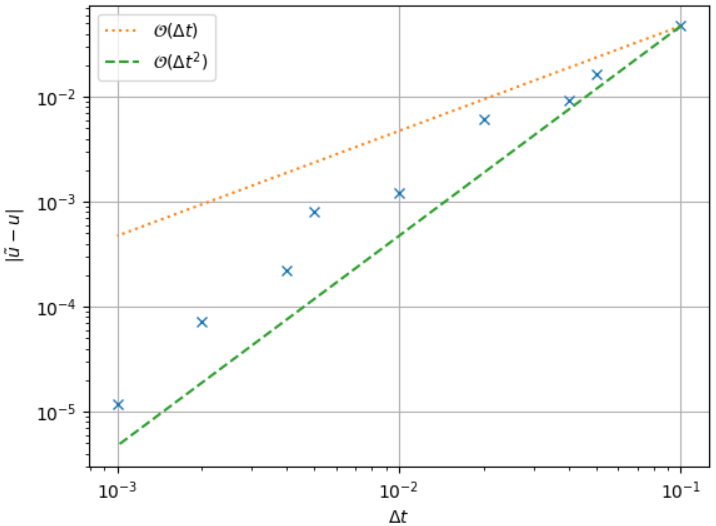
\includegraphics[width=0.5\textwidth]{resources/fake_fluid.png}
    \caption{TODO: }
    \label{fig:fake-fluid}
\end{figure}

In Figure \ref{fig:fake-fluid} one can observe that the error decreases in a higher-order fashion, as previously observed by the single solver study. This rules out this adapter as the possible source of error, as it showed to give a good error convergence.

\subsection{Verification of fluid participant} \label{sec:fluid-part}
With the aim of verifying the fluid participant of the FSI simulation, we ran several single-solver simulations, only taking the fluid part of the scenario. The tested case could be seen as a channel with an inverse cavity that stands out, following the geometry of the flap. From this experiments, we observed that this setup was unstable for a high Courant–Friedrichs–Lewy (CFL) number, which is defined as $\text{CFL} = \frac{u \Delta t}{\Delta x}$. In the FSI simulation of section \label{sec:FSI}, we computed cases with a high CFL number when we had large time step sizes, which failed to converge in this test. With the aim of improving the stability of the simulation we tried initializing the velocity field with precomputed values of a simulation that reached a steady state.

Once we could obtain some stable simulations, we defined a time-dependent input velocity, so we could observe a decrease of the error when decreasing the time step size. Then, a convergence study of the error was performed, by running the same simulation with the Crank-Nicolson scheme, and only varying the time step size parameter. In Figure \ref{fig:fluid_test} we can observe the results of this study, showing how the error does not follow a higher order convergence. In fact, it's decreasing order is very similar than the one we observed in Figure \ref{fig:coupled_v2_v3} for the Crank-Nicolson scheme. This showcases that the fluid solver was the source of the poor error convergence.


% \section{OpenFOAM Adapter?}
% \begin{itemize}
%     \item Maybe explain a bit how it interacts with the solver, quite documented already by \href{https://precice.org/adapter-openfoam-extend.html}{Adapter documentation}, and by \href{https://journal.openfoam.com/index.php/ofj/article/view/88/78}{Article of Gerasimos et al.}.
%     \item Mention what should be fixed, maybe propose a prototype?
%     \item Mention how should be tested, with a fake-fluid setup for example. Then also test with the same setup to see if it is viable.
% \end{itemize}



\section{Conclusions and future work}

In this study, we examined the convergence behavior of open-source solvers, specifically OpenFOAM and CalculiX, in single-solver and fluid-structure interaction (FSI) simulations, using the preCICE coupling library. To do so, we developed a comprehensive pipeline to automate simulation execution and analysis, facilitating efficient exploration of various solver configurations. This allowed us to perform systematic convergence studies and result comparison across different scenarios. 

Our analysis yielded several key findings. Firstly, both OpenFOAM and CalculiX demonstrate the potential for achieving higher-order convergence in time stepping schemes when used independently. Through convergence studies, we established that higher-order accuracy is attainable in both fluid dynamics and structural mechanics simulations, when suitable solver configurations and scenarios are employed.
Moreover, we achieved a linear decrease in the error when using first-order timestepping methods on coupled simulations with preCICE. However, challenges arose in maintaining the higher-order in FSI simulations. Through meticulous analysis and verification tests, we identified the fluid participant as a major error source contributing to these discrepancies. Simultaneously, we verified the correct behaviour of the preCICE adapter for CalculiX. This reflected that the used perpendicular flap scenario was not adequate to achieve a higher-order convergence with OpenFOAM. Even though, we leave as future work the thorough testing of this setup utilizing other solvers, which provide different higher-order timestepping schemes that might be more robust than the Crank-Nicolson. Exploring alternative physical configurations with lower CFL numbers would also be interesting, as it would provide better stability and facilitate the execution of convergence studies. Scenarios with finner spatial discretization could also help to observe a better error convergence, as the spatial error contribution would not be dominat until smaller scales. 

Overall, this study offers valuable insights into the convergence behavior of open-source solvers, and serves as ground work for achieving more accurate coupled simulations.


\pagebreak

\printbibliography

\end{document}
